\documentclass{beamer}

\usepackage{epsfig}
\usepackage{multicol}
\usepackage{geometry}
%\usepackage[dvipsnames]{xcolor}
\usepackage{textcomp}
\usepackage{graphicx}
\usepackage{caption}
\usepackage{subcaption}
\usepackage{amsmath}
\usepackage{tcolorbox}
\usetheme{Boadilla}
\usepackage{pict2e}
\usepackage{tikz}
\usepackage{xcolor}


\title[Traitement du signal numérique]{Traitement du signal numérique - HEI4 IMS}
\author[Antony Bazir]{}

\setlength{\unitlength}{1cm}

\begin{document}
\section{Signaux Biomédicaux}
\subsection{Types de signaux}
\begin{frame}
\frametitle{Signaux Biomédicaux}
Différents types de signaux biomédicaux: \\
\vspace{0.3cm}
\begin{itemize}
\item<2-> Bioéléctriques
\vspace{0.2cm}
\item<3-> Bioimpédances
\vspace{0.2cm}
\item<4-> Bioacoustiques
\vspace{0.2cm}
\item<5-> Biomagnétiques
\vspace{0.2cm}
\item<6-> Biochimiques
\vspace{0.2cm}
\item<7-> Biooptiques
\end{itemize}
\end{frame}

\begin{frame}
\frametitle{Signaux Bioélectriques}
\textbf{Potentiel électrochimique de membrane}
\begin{columns}
\column{60mm}
 \includegraphics[scale=0.2]{membrane_ions.png}
 \footnotesize \textit{Najarian \& Splinter, 2005}
\column{60mm}
\begin{itemize}
\item ions = potentiel électrique à travers la membrane
\vspace{0.2cm}
\item -70 mV et -40 mV par cellules
\vspace{0.2cm}
\item Peut fournir de l'énergie 
\vspace{0.2cm}
\item Utilisé par les cellules nerveuses et musculaires pour leur fonctionnement
\vspace{0.2cm}
\item Mesuré par le biais d'électrodes sur une ou plusieurs cellules
\end{itemize}
\end{columns}
\end{frame}

\begin{frame}
\frametitle{Bioimpédances}
\textbf{\underline{Impédance}} : Extension de la notion de résistance aux tensions/courants alternatifs 
\begin{columns}
\column{60mm}
\begin{center}
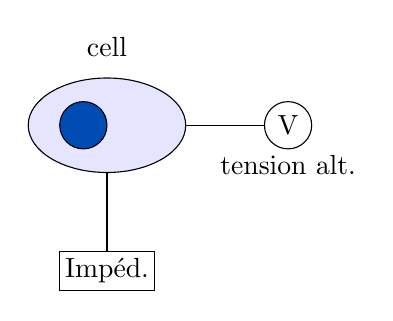
\begin{tikzpicture}
\draw (0,1) node{cell};
\draw[fill=blue!10!white] (0,0) ellipse (1 and 0.6);
\draw[fill=blue!70!green] (-0.3,0) circle(0.3);
\draw(1,0)--(2,0); 
\draw (2.3,0) circle(0.3) node{V};
 \draw (2.3,-0.5) node{tension alt.};
 \draw(0,-0.6)--(0,-1.6); 
 \draw (-0.6,-2.1) rectangle node[text centered]{Impéd.} (0.6,-1.6) ;
\end{tikzpicture} 
\end{center}
\column{60mm}
\begin{itemize}
\item Envoi d'une tension alternative dans le tissu ou la cellule
\vspace{0.2cm}
\item La résistance mesurée informe sur l'état du tissu
\vspace{0.2cm}
\item Fréquence : 50 kHz - 1 MHz 
\vspace{0.2cm}
\item Courant: 2 - 20 mA 
\end{itemize}
\end{columns} 
\end{frame}

\begin{frame}
\frametitle{Signaux Bioacoustiques}
\textbf{Ondes mécaniques/acoustiques émises par le corps}
\begin{columns}
\column{60mm}
\begin{center}
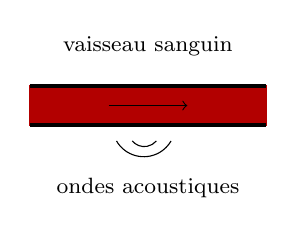
\begin{tikzpicture}
\draw (1.5,1) node[text centered]{\footnotesize vaisseau sanguin};
\draw[red!70!black,fill=red!70!black] (0,0) rectangle (3,0.5);
\draw[ultra thick] (0,0.5)--(3,0.5);
\draw[ultra thick] (0,0)--(3,0);
\draw[->] (1,0.25)--(2,0.25);

\draw (1.3,-0.2)arc (220:320:0.2);
\draw (1.1,-0.2)arc (210:330:0.4);
\draw (1.5,-0.8) node[text centered]{\footnotesize ondes acoustiques};
\end{tikzpicture} 
\end{center}
\textit{Exemple d'ondes acoustiques émises par le corps.}
\column{60mm}
\begin{itemize}
\item Peuvent informer sur la fonction d'un organe
\vspace{0.2cm}
\item Fréquence : 100-1000 Hz 
\vspace{0.2cm}
\item Mesuré par le biais de traducteurs acoustiques
\end{itemize}
\end{columns}
\end{frame}
%https://sigport.org/topic-tags/bioacoustics-and-medical-acoustics pour les exemples

\begin{frame}
\frametitle{Signaux Biomagnétiques}
\textbf{Courants électriques $\rightarrow$ Champ magnétique}
\begin{columns}
\column{60mm}
\vspace{0.2cm}\\
 \includegraphics[scale=0.3]{biomag_sig.png}\\
 \vspace{0.1cm}
 \textit{B.J. Roth, MDPI, 2023}
\column{60mm}
\begin{itemize}
\item Champs magnétiques faibles 1-100 pT (champ terrestre $\approx$  \textmu T)
\vspace{0.2cm}
\item Fréquence 0.1-1000 Hz
\vspace{0.2cm}
\item Mesuré avec des magnétomètres (bobines)
\vspace{0.2cm}
\item Utile au diagnostic de certaines pathologies neurologiques (epilepsie etc...)
\end{itemize}

\end{columns}
\end{frame}

\begin{frame}
\frametitle{Signaux Biomécaniques}
\textbf{Mouvements issus d'actions/contraintes mécaniques}
\begin{columns}
\column{60mm}
 \includegraphics[scale=0.33]{gait.png}\\
 \vspace{0.1cm}
 \textit{Mezghani et al., IEEE, 2016}

\column{60mm}
\begin{itemize}
\item Fréquence : 0.001 - 1 Hz
\vspace{0.2cm}
\item Mesures de force, vitesse ou accélération 
\vspace{0.2cm}
\item Pas de propagation $\rightarrow$ mesure potentiellement invasive
\vspace{0.2cm}
\end{itemize}
\end{columns}
\end{frame}

\begin{frame}
\frametitle{Signaux Biochimiques}
\begin{columns}
\column{60mm}
 \includegraphics[scale=0.5]{ABG.png}\\
 \vspace{0.1cm}
 \textit{Cleveland Clinic, 2022}
\column{60mm}
\begin{itemize}
\item Estimation de concentrations
\vspace{0.2cm}
\item Signaux variant généralement très lentement
\end{itemize}
\end{columns}
\end{frame}

\begin{frame}
\frametitle{Signaux Biooptiques}
\textbf{Informations basées sur la détection de lumière ou les propriétés optiques}
\begin{columns}
\column{60mm}
 \includegraphics[scale=0.15]{pox.png}\\
 \vspace{0.1cm}
 \textit{Fonctionnement d'un oxymètre, wikipedia.org}
\column{60mm}
\begin{itemize}
\item Mesures spectrales (différentes longueurs d'onde)
\vspace{0.2cm}
\item Détecter avec des capteurs CMOS ou des photodiodes 
\vspace{0.2cm}
\item Signaux sujets à la diffusion et à la réfraction
\end{itemize}
\end{columns}
\end{frame}

\begin{frame}
\frametitle{Caractéristiques des signaux biomédicaux déterministes}
\begin{center}
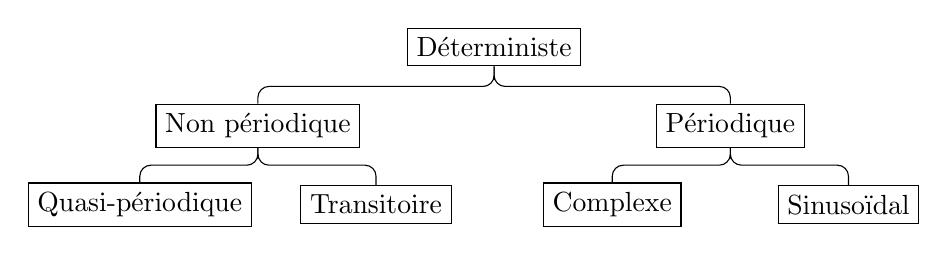
\begin{tikzpicture}
\node[draw,rectangle] (D) at (0,0) {Déterministe};


\node[draw,rectangle] (NP) at (-3,-1) {Non périodique};
\node[draw,rectangle] (P) at (3,-1) {Périodique};
\draw[rounded corners] (D) |- (0,-0.5) -| (NP);
\draw[rounded corners] (D) |- (0,-0.5) -| (P);


\node[draw,rectangle] (S) at (4.5,-2) {Sinusoïdal};
\node[draw,rectangle] (C) at (1.5,-2) {Complexe};
\draw[rounded corners] (P) |- (3,-1.5) -| (S);
\draw[rounded corners] (P) |- (3,-1.5) -| (C);

\node[draw,rectangle] (Q) at (-4.5,-2) {Quasi-périodique};
\node[draw,rectangle] (T) at (-1.5,-2) {Transitoire};
\draw[rounded corners] (NP) |- (-3,-1.5) -| (Q);
\draw[rounded corners] (NP) |- (-3,-1.5) -| (T);
\end{tikzpicture}
\end{center}
\end{frame}

\subsection{Déterministes vs. Stochastiques}
\begin{frame}
\frametitle{Caractéristiques des signaux biomédicaux déterministes}
\textbf{Déterministe }: Peut être prédit et/ou décrit quasi-exactement par une fonction.
\vspace{0.1cm}
\begin{itemize}
\item \textbf{Périodique} 
\vspace{0.1cm}
\begin{itemize}
 \item \textbf{Sinusoïdal:} Pure sinusoïde d'une fréquence et d'une phase donnée
 \vspace{0.1cm}
 \item \textbf{Complexe:} Combinaison d'au moins deux sinusoïdes pures 
\end{itemize}
 \vspace{0.2cm}
\item \textbf{Non-Périodique }
\begin{itemize}
 \vspace{0.1cm}
 \item \textbf{Quasi-Périodique}
 \vspace{0.1cm}
 \item \textbf{Transitoire} : Croissance/Décroissance monotone
\end{itemize}
\end{itemize}
\end{frame}

\begin{frame}
\frametitle{Caractéristiques des signaux biomédicaux stochastiques}
\begin{center}
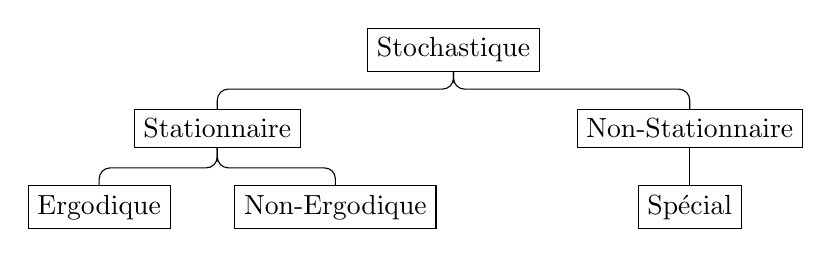
\begin{tikzpicture}

\node[draw,rectangle] (S) at (0,0) {Stochastique};

\node[draw,rectangle] (ST) at (-3,-1) {Stationnaire};
\node[draw,rectangle] (NS) at (3,-1) {Non-Stationnaire};
\draw[rounded corners] (S) |- (0,-0.5) -| (ST);
\draw[rounded corners] (S) |- (0,-0.5) -| (NS);


\node[draw,rectangle] (E) at (-4.5,-2) {Ergodique};
\node[draw,rectangle] (NE) at (-1.5,-2) {Non-Ergodique};
\draw[rounded corners] (ST) |- (-3,-1.5) -| (E);
\draw[rounded corners] (ST) |- (-3,-1.5) -| (NE);

\node[draw,rectangle] (SP) at (3,-2) {Spécial};
\draw[rounded corners] (NS) |- (3,-1.5) -| (SP);

\end{tikzpicture}
\end{center}
\end{frame}

\begin{frame}
\frametitle{Caractéristiques des signaux biomédicaux stochastiques}
\textbf{Stochastique} :  \'Evolution, discrète ou à temps continu, d'une variable aléatoire décrit par des variables statistiques
\vspace{0.2cm}
\begin{itemize}
\item \textbf{Stationnaire:} Les variables statistiques (moyenne variance etc...) sont constantes au cours du temps 
\vspace{0.1cm}
\begin{itemize}
 \item \textbf{Ergodique}:  processus stochastique pour lequel les statistiques peuvent être approchées par l'étude d'une seule réalisation suffisamment longue. 
 \vspace{0.1cm}
 \item \textbf{Non-Ergodique}
\end{itemize}
\vspace{0.2cm}
\item \textbf{Non-Stationnaire}
\vspace{0.1cm}
\begin{itemize}
 \item \textbf{Spécial}
\end{itemize}
\end{itemize}
\end{frame}

\subsection{Exemples de signaux}
\subsubsection{\'Electrocardiogramme}
\begin{frame}
\frametitle{Exemple de signaux : \'Electrocardiogramme (ECG) }
\begin{columns}
\column{60mm}
\includegraphics[scale=0.4]{heart.png}\\
\textit{\footnotesize Schéma du coeur avec ses pacemakers naturels, Najarian \& Splinter}
\column{60mm}
\begin{itemize}
\item Les noeuds "activent" les cellules cardiaques
\vspace{0.5cm}
\item Le changement de potentiel sur l'ensemble de cellules se propage. 
\vspace{0.3cm}
\item On mesure ce potentiel en différents points du corps à la surface de la peau 
\end{itemize}
\end{columns}
\end{frame}

\begin{frame}
\frametitle{Exemple de signaux : \'Electrocardiogramme (ECG)}
\begin{center}
\includegraphics[scale=0.35]{PQRSTU.png}\\
\textit{\footnotesize (a) Forme caractéristique d'un ECG. (b) ECG d'un patient normal. Najarian \& Splinter}
\end{center}
\begin{itemize}
\item Le signal correspond aux polarisations/dépolarisations de différentes parties du coeur.
\item Chaque partie du signal a une durée de $\approx$ 100 ms
\item Signal quasi-périodique
\end{itemize}
\end{frame}

\begin{frame}
\frametitle{Exemple de signaux : \'Electrocardiogramme (ECG)}
\begin{center}
\includegraphics[scale=0.35]{PQRSTU.png}\\
\textit{\footnotesize (a) Forme caractéristique d'un ECG. (b) ECG d'un patient normal. Najarian \& Splinter}
\end{center}
Analyses: 
\vspace{0.1cm}
\begin{itemize}
\item Détermination du rythme cardiaque
\vspace{0.1cm}
\item Contenu fréquentiel des signaux
\vspace{0.1cm} 
\item Analyse en ondelettes
\end{itemize}
\end{frame}

\begin{frame}
\frametitle{Exemple de signaux : \'Electrocardiogramme (ECG)}
\begin{center}
\includegraphics[scale=0.3]{chaine_ECG.png}\\
\textit{\footnotesize Exemple chaîne de traitement d'un ECG Tompkins, 2000}
\end{center}
\begin{enumerate}
\item 1ère étape de filtrage analogique
\item Conversion en numérique en vue d'analyse et de post-traitement
\end{enumerate}
\end{frame}

\begin{frame}
\frametitle{Exemple de signaux : \'Electrocardiogramme (ECG)}
\begin{center}
\includegraphics[scale=0.35]{tr_num_ecg.png}\\
\textit{\footnotesize Algorithme de détection du complexe QRS, Tompkins, 2000}\\
\end{center}
Filtrage temps réel du signal numérique \& Extraction du QRS
\begin{enumerate}
\item<2-> filtrage passe-bande pour ne garder que les fréquences du QRS
\item<3-> Dérivée du signal (QRS = forte pente)
\item<4-> Mise au carré (signal positif et haute fréquences accentuées)
\item<5-> Moyennage
\end{enumerate}
\only<6->{On reviendra sur cette chaine de traitement plus en détail...}
\end{frame}

\subsubsection{\'Electroencéphalogramme}
\begin{frame}
\frametitle{Exemple de signaux : \'Electroencéphalogramme (EEG)}
\begin{center}
\includegraphics[scale=0.35]{EEG_electrodes.png}\\
\textit{\footnotesize Placement des électrodes pour un EEG. Najarian \& Splinter}
\end{center}
\vspace{0.2cm}
\begin{itemize}
\item Amplification des signaux de polarisation/dépolarisation des cellules nerveuses
\item On mesure généralement des potentiels évoqués par des stimuli
\end{itemize}

\end{frame}

\begin{frame}
\frametitle{Exemple de signaux : \'Electroencéphalogramme (EEG)}
\begin{columns}
\column{60mm}
\includegraphics[scale=0.33]{EEG.png}\\
\textit{\footnotesize Signaux EEG. Najarian \& Splinter}
\column{60mm}
\begin{itemize}
\item Signaux stochastiques 
\vspace{0.2cm}
\item Analyse spectral : Détection des ondes $\alpha$, $\beta$, $\delta$ et $\theta$
\vspace{0.2cm}
\item Analyse dans le domaine temporel pour les potentiels évoqués
\end{itemize}
\end{columns}
\end{frame}

\begin{frame}
\frametitle{Exemple de signaux : \'Electroencéphalogramme (EEG)}
\begin{columns}
\column{60mm}
\includegraphics[scale=0.33]{evp_eeg.png}\\
\textit{\footnotesize Signaux EEG avec stimuli. Najarian \& Splinter}
\column{60mm}
Dans ce cas, on va vouloir détecter le signal dans le domaine temporel
\end{columns}

\end{frame}

\begin{frame}
\frametitle{Exemple de signaux : \'Electroencéphalogramme (EEG)}
\begin{columns}
\column{60mm}
\includegraphics[scale=0.3]{evp_moy.png}\\
\textit{\footnotesize Moyennage d'un EEG avec stimuli. Bronzino, 2010}
\column{60mm}
\begin{itemize}
\item Signal brut très bruité $\rightarrow$ stimuli difficilement identifiable
\vspace{0.2cm}
\item Le bruit est de nature stochastique 
\vspace{0.2cm}
\item Le signal se reproduit environ toujours au même temps
\vspace{0.2cm}
\item Le moyennage amplifie le signal et élimine le bruit.
\end{itemize}
\end{columns}

\end{frame}

\subsubsection{Ultrasons}
\begin{frame}
\frametitle{Exemple de signaux : Ultrasons}
\begin{columns}
\column{60mm}
\includegraphics[scale=0.23]{Ultrasonic.png}\\
\textit{\footnotesize Principe d'imagerie ultrasonore. Hazari, 2010}
\column{60mm}
\begin{enumerate}
\item<2-> \textbf{\'Emission} ultrasonore vers la zone d'intérêt
\vspace{0.2cm}
\item<3-> \textbf{Détection} du signal ultrasonore transmis, réfléchi ou diffusé
\vspace{0.2cm}
\item<4-> \textbf{Traitement/Analyse} du signal reçu
\end{enumerate}
\end{columns}
\end{frame}


\begin{frame}
\frametitle{Exemple de signaux : Ultrasons}
\begin{columns}
\column{60mm}
\includegraphics[scale=0.23]{A-scan.png}\\
\textit{\footnotesize A-scan en imagerie ultrasonore. Hazari, 2010}
\column{60mm}
Pour un traducteur unique:
\vspace{0.2cm}
\begin{enumerate}
\item<2-> \'Emission du signal par excitation électrique
\vspace{0.2cm}
\item<3-> Propagation et réflexions aux interfaces 
\vspace{0.2cm}
\item<4-> Réception par le traducteur
\end{enumerate}
\vspace{0.2cm}
\only<4->{\textbf{Unité de base de l'imagerie ultrasonore}}
\end{columns}
\end{frame}

\begin{frame}
\frametitle{Exemple de signaux : Ultrasons}
\begin{center}
\includegraphics[scale=0.25]{B-scan.png}\\
\textit{\footnotesize B-scans en imagerie ultrasonore. Hazari, 2010}\\
\end{center}
On dispose généralement d'un réseau de traducteurs qui vont former les pixels de l'image\\
\vspace{0.2cm}
\begin{enumerate}
\item<2-> \textbf{Conversion} des A-scans en niveau de gris
\vspace{0.2cm}
\item<3-> \textbf{Cartographie spatiale} des signaux résultants 
\end{enumerate}
\vspace{0.2cm}

\end{frame}

\begin{frame}
\frametitle{Exemple de signaux : Ultrasons}
\textbf{Chaine de traitement pour les signaux ultrasonores}\\
\begin{center}
\includegraphics[scale=0.33]{chaine_us.png}\\
\textit{\footnotesize Chaîne de traitement en imagerie ultrasonore. Hazari, 2010}\\
\end{center}
\begin{itemize}
\item<2-> Premier filtrage analogique 
\item<3-> Conversion en numérique
\item<4-> Traitements mathématiques numériques 
\end{itemize}
\end{frame}

\begin{frame}
\frametitle{Exemple de signaux : Ultrasons}
\begin{columns}
\column{60mm}
\includegraphics[scale=0.23]{Ultrasonic.png}\\
\textit{\footnotesize Principe d'imagerie ultrasonore. Hazari, 2010}
\column{60mm}
Applications:
\begin{itemize}
\item Imagerie de contraste $\rightarrow$ variation \textbf{relative} prop. méca\\
\begin{itemize}
\item Détection de discontinuité/interfaces 
\end{itemize}
\vspace{0.2cm}
\item Mesure \textbf{absolue} prop. méca 
\begin{itemize}
\item Mesure pulse-écho  
\item Mesure régime sinusoïdal
\end{itemize}
\vspace{0.2cm}
\item \textbf{Cartographie} propriétés mécaniques
\begin{itemize}
\item carte vitesse du son 
\item carte atténuation
\end{itemize}
\end{itemize}
\end{columns}
\end{frame}

\subsubsection{Rayons-X/$\gamma$}
\begin{frame}
\frametitle{Exemple de signaux : Rayons-X/$\gamma$}
Principe :
\[  I = I_0 \cdot \exp (- \int^{x_{max}}_{x_0} \; \mu (Z(x),E) \; dx)  \] 
\vspace{0.5cm}
\begin{itemize}
\item $I_0, I$: intensités initiale et détectée 
\item $x_0, x_{max}$ : Points d'entrée et de sortie de l'objet à imager
\item $Z(x)$  numéro atomique du matériau traversé 
\item $E$ énergie du rayonnement émis
\end{itemize}
\vspace{0.5cm}
\only<2->{
\textbf{Offre un contraste entre différents tissus}
}
\end{frame}

\begin{frame}
\frametitle{Exemple de signaux : Rayons-X/$\gamma$}
\begin{columns}
\column{60mm}
\begin{center}
\includegraphics[scale=0.12]{xray_plan.jpg}\\
\textit{Radiographie pulmonaire numérisée, Nevit Delmen}
\end{center}
\column{60mm}
\begin{center}
\includegraphics[scale=0.22]{xray_tomo.png}\\
\textit{Tomographie axiale calculée, Mustafa Mafraji}
\end{center}
\end{columns}
\end{frame}

\begin{frame}
\frametitle{Exemple de signaux : Rayons-X/$\gamma$}
\begin{center}
\includegraphics[scale=0.3]{dig_mammo.png}\\
\end{center}
\begin{itemize}
\item Radiographie numérique : Comptage de photons/mesure d'énergie $\rightarrow$ signal numérique
\item Standard actuel dans le domaine médical
\item Outils de traitement d'image numérique disponible
\end{itemize}
\end{frame}

\begin{frame}
\frametitle{Exemple de signaux: résumé}
\begin{itemize}
\item \textbf{\'Electrocardiogramme }
\begin{itemize}
\item signal bioélectrique
\item Analyse fréquentielle 
\item Détection de motifs (QRS, RR, etc...)
\end{itemize}
\vspace{0.1cm}
\item \textbf{\'Electroencéphalogramme}
\begin{itemize}
\item signal bioélectrique
\item Analyse fréquentielle (ondes $\alpha$, $\beta$, $\delta$...) 
\item Détection de motifs (ondes évoquées)
\end{itemize}
\vspace{0.1cm}
\item  \textbf{Ultrasons} 
\begin{itemize}
\item signal acoustique
\item mesure des propriétés acoustiques  (rigidité, etc...)
\item imagerie de contraste (échographie, tomographie, etc...)
\end{itemize}
\vspace{0.1cm}
\item \textbf{Rayons-X/$\gamma$}
\begin{itemize}
\item signal electromagnétique
\item imagerie de contraste (échographie, tomographie, etc...)
\end{itemize}
\end{itemize} 
\end{frame}

\subsection{Chaîne d'instrumentation Numérique}
\begin{frame}
\frametitle{Chaine d'instrumentation Numérique}
\begin{center}
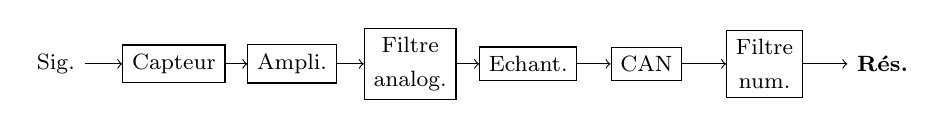
\begin{tikzpicture}
\node (S) at (0,0) {\footnotesize  Sig.};
\node[draw,rectangle,align=center]  (C) at (1.5,0) {\footnotesize Capteur}; 
\node[draw,rectangle,align=center]  (A) at (3,0) {\footnotesize Ampli.}; 
\node[draw,rectangle,align=center]  (F) at (4.5,0) {\footnotesize Filtre \\ \footnotesize analog.}; 
\node[draw,rectangle,align=center]  (E) at (6,0) {\footnotesize Echant.}; 
\node[draw,rectangle,align=center]  (AD) at (7.5,0) {\footnotesize CAN}; 
\node[draw,rectangle,align=center]  (N) at (9,0) {\footnotesize Filtre \\ \footnotesize num.}; 
\node (R) at (10.5,0) {\footnotesize  \textbf{Rés.}};

\draw[->] (S)--(C);
\draw[->] (C)--(A);
\draw[->] (A)--(F);
\draw[->] (F)--(E);
\draw[->] (E)--(AD);
\draw[->] (AD)--(N);
\draw[->] (N)--(R);
\end{tikzpicture}
\end{center}
\begin{enumerate}
\item Conversion du signal physique en tension
\item Amplification
\item Filtrage analogique
\item \'Echantillonnage  (Bloqueur)
\item Conversion analogique-numérique
\item Filtrage numérique 
\end{enumerate}
\vspace{0.3cm}
\only<2->{
Des variantes existent...
}
\end{frame}

\begin{frame}
\frametitle{Chaine d'instrumentation Numérique : Capteur}
\begin{center}
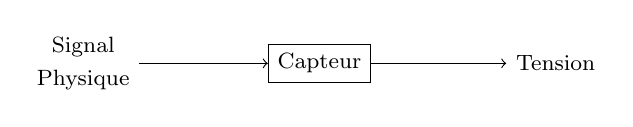
\begin{tikzpicture}
\node[align=center] (S) at (0,0) {\footnotesize  Signal\\ \footnotesize  Physique};
\node[draw,rectangle,align=center]  (C) at (3,0) {\footnotesize Capteur};
\node[align=center] (T) at (6,0) {\footnotesize  Tension};

\draw[->] (S)--(C);
\draw[->] (C)--(T);
\end{tikzpicture}
\end{center}
\vspace{0.1cm}
\textbf{Caractéristiques :}\\
\vspace{0.1cm}
\begin{itemize}
\item Conversion \textbf{univoque} entre le signal physique et la tension
\vspace{0.1cm}
\item Gamme de mesure et/ou Plage de linéarite
\item \textbf{Résolution} spatiale et temporelle
\item Exemples : 
\begin{itemize}
\item Tradcuteur piézoélectrique
\item Détecteur à comptage de photons
\item Electrodes ECG/EEG
\end{itemize}
\vspace{0.1cm}
\end{itemize}
\end{frame}

\begin{frame}
\frametitle{Chaine d'instrumentation Numérique : Amplificateur}
\begin{center}
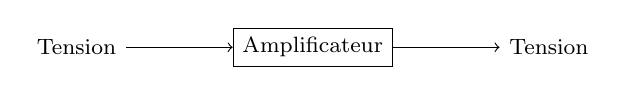
\begin{tikzpicture}
\node[align=center] (S) at (0,0) {\footnotesize  Tension};
\node[draw,rectangle,align=center]  (C) at (3,0) {\footnotesize Amplificateur};
\node[align=center] (T) at (6,0) {\footnotesize  Tension};

\draw[->] (S)--(C);
\draw[->] (C)--(T);
\end{tikzpicture}
\end{center}
\vspace{0.1cm}
\textbf{Caractéristiques :}\\
\vspace{0.1cm}
\begin{itemize}
\item \textbf{Applique un facteur multplicatif sur le signal du capteur}
\vspace{0.1cm}
\item Adapte la tension à la gamme de CAN
\vspace{0.1cm}
\item Doit être \textbf{linéaire en tension ET en fréquence}
\vspace{0.1cm}
\item Amplifie également le bruit 
\vspace{0.1cm}
\begin{itemize}
\item nécessité potentielle d'un premier filtrage 
\vspace{0.1cm}
\item  filtre notch 50 Hz...
\end{itemize}
\end{itemize}
\end{frame}

\begin{frame}
\frametitle{Chaine d'instrumentation Numérique : Filtrage analogique}
\begin{center}
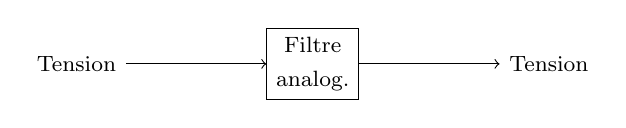
\begin{tikzpicture}
\node[align=center] (S) at (0,0) {\footnotesize  Tension};
\node[draw,rectangle,align=center]  (C) at (3,0) {\footnotesize Filtre \\ \footnotesize analog.};
\node[align=center] (T) at (6,0) {\footnotesize  Tension};

\draw[->] (S)--(C);
\draw[->] (C)--(T);
\end{tikzpicture}
\end{center}
\vspace{0.1cm}
\textbf{Caractéristiques :}\\
\vspace{0.2cm}
\begin{itemize}
\item \textbf{Souvent utilisé pour éliminer des parasites bien identifiés }
\vspace{0.2cm}
\begin{itemize}
\item Passe-bas : Bruit des électrodes (EEG/ECG)
\vspace{0.2cm}
\item Notch : élimination du 50-60 Hz
\vspace{0.2cm}
\item Passe-haut : élimination de la respiration/mouvments corporels (ultrasons)
\end{itemize}
\end{itemize}
\end{frame}

\begin{frame}
\frametitle{Chaine d'instrumentation Numérique : \'Echantillonnage}
\begin{center}
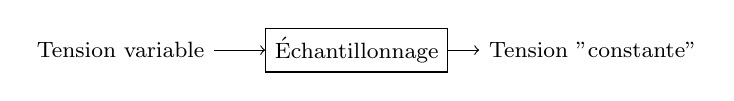
\begin{tikzpicture}
\node[align=center] (S) at (0,0) {\footnotesize  Tension variable};
\node[draw,rectangle,align=center]  (C) at (3,0) {\footnotesize \'Echantillonnage};
\node[align=center] (T) at (6,0) {\footnotesize  Tension "constante"};

\draw[->] (S)--(C);
\draw[->] (C)--(T);
\end{tikzpicture}
\end{center}
\vspace{0.1cm}
\textbf{\textbf{Circuit bloqueur} :}\\
\vspace{0.2cm}
\begin{itemize}
\item \textbf{Prend la valeur en  entrée et la maintient pendant $T_e$ }
\vspace{0.2cm}
\begin{itemize}
\item Retard d'ouverture 
\vspace{0.2cm}
\item Incertitude d'ouverture 
\vspace{0.2cm}
\item Temps d'établissement du blocage
\end{itemize}
\vspace{0.2cm}
\item Temps caractéristiques \textbf{bien inférieurs} à la période d'échantillonnage.
\end{itemize}
\end{frame}

\begin{frame}
\frametitle{Chaine d'instrumentation Numérique : Conversion Analogique/Numérique}
\begin{center}
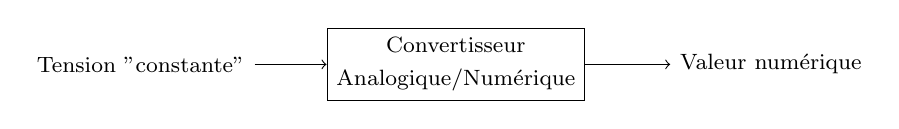
\begin{tikzpicture}
\node[align=center] (S) at (0,0) {\footnotesize  Tension "constante"};
\node[draw,rectangle,align=center]  (C) at (4,0) {\footnotesize Convertisseur \\ \footnotesize  Analogique/Numérique};
\node[align=center] (T) at (8,0) {\footnotesize  Valeur numérique};

\draw[->] (S)--(C);
\draw[->] (C)--(T);
\end{tikzpicture}
\end{center}
\vspace{0.1cm}
\begin{itemize}
\item \textbf{Convertit la valeur réelle en valeur binaire}
\vspace{0.2cm}
\begin{itemize}
\item Gamme dynamique divisé en N échelons  
\vspace{0.2cm}
\item Valeur réelle située dans un échelon pendant $T_e$
\vspace{0.2cm}
\item Correspondance à une valeur numérique (00011..)
\end{itemize}
\vspace{0.2cm}
\item Plusieurs architectures possibles (Double rampe, Sigma-delta...) basées sur des cycles de charge-décharges suivies dans le temps
\end{itemize}
\end{frame}

\begin{frame}
\frametitle{Filtrage numérique :  Extraction du complexe QRS}
\begin{center}
\includegraphics[scale=0.35]{tr_num_ecg.png}\\
\textit{\footnotesize Algorithme de détection du complexe QRS, Tompkins, 2000}\\
\end{center}
Filtrage temps réel du signal numérique \& Extraction du complexe QRS\\
\vspace{0.3cm}
Pourquoi extraire le complexe QRS ?\\
\vspace{0.2cm}
\begin{itemize}
\item suivi de la condition du patient en temps réel 
\item Etablissement des tachogrammes (RR)
\item \'A la base de beacoup d'algorithmes acutels...
\end{itemize}

\end{frame}

\begin{frame}
\frametitle{Filtrage numérique :  Extraction du complexe QRS}
\textbf{Caractéristiques du complexe QRS}
\begin{center}
\includegraphics[scale=0.35]{QRS.png}\\

\end{center}
\underline{Origine physique} : dépolarisation des ventricules\\
\vspace{0.3cm}
Caractéristiques: \\
\vspace{0.1cm}
\begin{itemize}
\item Durée :  80 -100 ms
\item Fréquence : 10-15 Hz 
\end{itemize}

\end{frame}

\begin{frame}
\frametitle{Filtrage numérique :  Extraction du complexe QRS}
\begin{center}
\includegraphics[scale=0.3]{ECG_spectrum.png}\\
\textit{\scriptsize Spectre en amplitude de l'ECG, Tompkins,2000}\\
\vspace{0.1cm}
\end{center}
Importance du filtrage passe-bande...
\end{frame}

\begin{frame}
\frametitle{Filtrage numérique :  Extraction du complexe QRS}
\begin{center}
\includegraphics[scale=0.3]{ECG_spectrum.png}\\
\textit{\scriptsize Spectre en amplitude de l'ECG, Tompkins,2000}\\
\vspace{0.1cm}
\end{center}
Comment choisir $T_e$ ? \only<2-> {Shannon $\rightarrow f_e > 80 Hz$  \only<3->{ Dans les faits, $f_e$ 500 Hz} }


\end{frame}

\begin{frame}
\frametitle{Détection QRS: Filtrage passe-bande}
\begin{center}
\includegraphics[scale=0.35]{tr_num_ecg.png}\\
\textit{\footnotesize Algorithme de détection du complexe QRS, Tompkins, 2000}\\
\vspace{0.3cm}
\end{center}
Filtrage temps réel du signal numérique \& Extraction du QRS
\begin{enumerate}
\item \textbf{filtrage passe-bande numérique}
\item Dérivée 
\item Mise au carré 
\item Moyennage
\end{enumerate}
\end{frame}

\begin{frame}
\frametitle{Détection QRS: Filtrage passe-bande}
 \textbf{Filtrage passe-bande numérique}\\
 \vspace{0.3 cm}
 Plusieurs méthodes possibles (liste non-exhasutive) :\\
 \vspace{0.2cm}
 \begin{itemize}
 \item Filtre récursifs à  2 pôles
 \vspace{0.2cm}
 \item Filtre à coefficients "entiers"
 \vspace{0.2cm}
 \end{itemize}
\end{frame}

\begin{frame}
\frametitle{Détection QRS: Filtrage passe-bande}
 \textbf{Filtrage passe-bande numérique: Filtre récursif à  2 pôles}\\
 \vspace{0.3 cm}
 Forme possible de la fonction de transfert :
 \[H(z) = \frac{c_1}{z-p_1} + \frac{c_2}{z-p_2} \]\\
  \vspace{0.3 cm}
  \'Equation aux différences :
 \[y[n] = b_1 y[n-1] - b_2 y[n-2] + x[n] - x[n-2] \]  
\end{frame}

\begin{frame}
\frametitle{Détection QRS: Filtrage passe-bande}
 \textbf{Filtrage passe-bande numérique: Filtre récursif à  2 pôles}\\

  Forme de l'équation aux différences :
 \[y[n] = b_1 y[n-1] - b_2 y[n-2] + x[n] - x[n-2] \]  \\
  \vspace{0.3 cm}
  Fonction de transfert :
   \[H(z) = \frac{1 - z^{-2}}{1 - b_1 z^{-1} + b_2 z^{-2}} \]  \\
  \vspace{0.3cm}
 \textbf{Comment se comporte ce filtre ?}
\end{frame}

\begin{frame}
\frametitle{Détection QRS: Filtrage passe-bande}
 \textbf{Filtrage passe-bande numérique: Filtre récursif à  2 pôles}\\

  \vspace{0.3 cm}
  Fonction de transfert :
   \[H(z) = \frac{1 - z^{-2}}{1 - b_1 z^{-1} + b_2 z^{-2}} \]  \\
  \vspace{0.3cm}
 On prend les valeurs données par Tompkins:
 \begin{itemize}
 \item $f_e$ = 500 Hz
 \item $b_1$ = 1.875
 \item $b_2$ = 0.9219
 \end{itemize}
\end{frame}

\begin{frame}
\frametitle{Détection QRS: Filtrage passe-bande}
 \textbf{Filtrage passe-bande numérique: Filtre récursif à  2 pôles}\\

  \vspace{0.3 cm}
  Fonction de transfert :
   \[H(z) = \frac{1 - z^{-2}}{1 - 1.875 z^{-1} + 0.9219 z^{-2}} \]  \\
  \vspace{0.3cm}
   \[H(z) = \frac{1 - e^{-4 j \pi \frac{f}{500}}}{1 - 1.875 e^{-2 j \pi \frac{f}{500}} + 0.9219  e^{-4 j \pi \frac{f}{500}}} \] 

\end{frame}

\begin{frame}
\frametitle{Détection QRS: Filtrage passe-bande}
 \textbf{Filtrage passe-bande numérique: Filtre récursif à  2 pôles}\\
\[H(z) = \frac{1 - e^{-4 j \pi \frac{f}{500}}}{1 - 1.875 e^{-2 j \pi \frac{f}{500}} + 0.9219  e^{-4 j \pi \frac{f}{500}}} \] 
\begin{center}
\begin{tikzpicture}
\begin{scope}[scale=2.5]
\draw[->] (0,0)-- (1.1,0)node[right] {\scriptsize $f$} ;
\draw[->] (0,0)-- (0,1.2)node[above] {\scriptsize  $|H(f)|$};
\draw[thick,blue] plot file {module_passebande1.txt};

\draw[dashed] (0.07,0) node[below]{\scriptsize 17 Hz}--(0.07,1);à
\draw[dashed] (1,0) node[below]{\scriptsize 250 Hz}--(1,0);
\end{scope}

\end{tikzpicture}
\end{center}
\vspace{0.3cm}
On sélectionne bien dans une gamme de fréquence autour du QRS
\end{frame}

\begin{frame}
\frametitle{Détection QRS: Filtrage passe-bande}
 \textbf{Filtrage passe-bande numérique: Filtre récursif à  2 pôles}\\
\begin{columns}
\column{60mm}
\[H(z) = \frac{1 - e^{-4 j \pi \frac{f}{500}}}{1 - 1.875 e^{-2 j \pi \frac{f}{500}} + 0.9219  e^{-4 j \pi \frac{f}{500}}} \]
\column{60mm} 
\begin{center}
\begin{tikzpicture}
\begin{scope}[scale=2.5]
\draw[->] (0,0)-- (1.1,0)node[right] {\scriptsize $f$} ;
\draw[->] (0,0)-- (0,1.2)node[above] {\scriptsize  $|H(f)|$};
\draw[thick,blue] plot file {module_passebande1.txt};

\draw[dashed] (0.07,0) node[below]{\scriptsize 17 Hz}--(0.07,1);à
\draw[dashed] (1,0) node[below]{\scriptsize 250 Hz}--(1,0);
\end{scope}

\end{tikzpicture}
\end{center}
\end{columns}
\vspace{0.3cm}
Remarques :
\begin{itemize}
\item Le numérateur sert à couper les basses fréquences
\item Coefficients optimisées pour augmenter la vitesse de calcul
\end{itemize}
\end{frame}

\begin{frame}
\frametitle{Détection QRS: Filtrage passe-bande}
 \textbf{Filtrage passe-bande numérique: Filtre à coeffs entiers}\\
\end{frame}
\end{document}
